% Bao cao cuoi ky mon Hoc may nang cao — dinh dang theo JTE-Template-Vie-01.2026
% Build: tectonic -X compile paper.tex --outdir build
\documentclass[11pt,a4paper]{article}

\usepackage{fontspec}
% font: Times clone tu bundle tectonic, du glyph tieng Viet
\setmainfont{texgyretermes}[Extension=.otf, UprightFont=*-regular,
  BoldFont=*-bold, ItalicFont=*-italic, BoldItalicFont=*-bolditalic]
\usepackage[a4paper,top=3cm,bottom=2.5cm,left=3cm,right=2cm,
            headheight=1cm,footskip=1.2cm]{geometry}
\usepackage{amsmath,amssymb}
\usepackage{graphicx}
\usepackage{array,booktabs,multirow}
\usepackage{enumitem}
\usepackage[hidelinks]{hyperref}
\usepackage{setspace}
\singlespacing

% doan van: thut dau dong 0,5cm; after 3pt; justified (mac dinh)
\setlength{\parindent}{0.5cm}
\setlength{\parskip}{3pt}
\emergencystretch=2em

% ---- tieu de cac cap (danh so tay theo yeu cau JTE) ----
\newcommand{\secvn}[1]{\vspace{6pt}\noindent\textbf{#1}\vspace{6pt}\par\nopagebreak}
\newcommand{\subsecvn}[1]{\vspace{6pt}\noindent\textbf{\textit{#1}}\vspace{6pt}\par\nopagebreak}
\newcommand{\subsubsecvn}[1]{\vspace{6pt}\noindent\textit{#1}\vspace{6pt}\par\nopagebreak}

% ---- caption hinh/bang: size 10, so hieu dam, tieu de nghieng ----
\newcommand{\figcap}[2]{\par\vspace{6pt}{\centering\fontsize{10}{12}\selectfont\textbf{Hình #1.} \textit{#2}\par}\vspace{6pt}}
\newcommand{\tabcap}[2]{{\raggedleft\fontsize{10}{12}\selectfont\textbf{Bảng #1.} \textit{#2}\par}\vspace{3pt}}

\begin{document}

% ============================ TIEU DE TIENG ANH ============================
\begin{center}
{\fontsize{13}{16}\selectfont\bfseries
Combining Multi-Layer Perceptron with Fuzzy Logic for Offensive Language Detection on Vietnamese Social Media Texts\par}
\vspace{6pt}
Anh Tu Phuong Nguyen$^{*}$\\
Ho Chi Minh City University of Technology and Education, Vietnam\\
$^{*}$Corresponding author. Email: 2611328@student.hcmute.edu.vn
\end{center}

\vspace{4pt}
\noindent\rule{\textwidth}{0.6pt}
\noindent
\begin{minipage}[t]{0.28\textwidth}
\vspace{2pt}
{\fontsize{10}{12}\selectfont
\textbf{ARTICLE INFO}\\[3pt]
Received: 21/7/2026\\
Revised:\\
Accepted:\\
Published:\\[6pt]
\textbf{KEYWORDS}\\[3pt]
Hate speech detection;\\
Fuzzy logic;\\
Multi-layer perceptron;\\
Vietnamese text classification;\\
Decision fusion.
}
\end{minipage}\hfill
\begin{minipage}[t]{0.68\textwidth}
\vspace{2pt}
{\fontsize{10}{12}\selectfont
\textbf{ABSTRACT}\\[3pt]
Offensive and hateful comments spread rapidly on Vietnamese social networks, while purely neural detectors act as black boxes and purely lexicon-based rules lack coverage. This study proposes FRF-MLP, a hybrid model that integrates a Mamdani fuzzy rule system into a Multi-Layer Perceptron for three-class offensive language detection (CLEAN, OFFENSIVE, HATE). An offensiveness lexicon is first learned from the training data by the log-odds ratio with informative Dirichlet prior; three document-level linguistic variables (maximum offensiveness, offensive-token density, and targeting degree) are then fuzzified by trapezoidal membership functions and evaluated by seven Mamdani rules. The fuzzy component is fused with the MLP at two levels: 22 fuzzy features are concatenated to the TF-IDF input, and the defuzzified class distribution is combined with the MLP posterior through a convex weight selected on the development set. Experiments on the ViHSD benchmark (33,398 human-annotated comments) show that FRF-MLP reaches 84.46\% accuracy and 62.95\% macro-F1, improving the plain MLP by +1.92 macro-F1 points and surpassing the published Text-CNN, GRU, and multilingual BERT baselines in macro-F1 while requiring no pre-training and training in minutes on a CPU. Ablation results confirm that both fusion levels contribute complementary gains, and the fuzzy component additionally provides rule-level interpretability.
}
\end{minipage}
\vspace{4pt}
\noindent\rule{\textwidth}{0.6pt}

% ============================ TIEU DE TIENG VIET ============================
\vspace{8pt}
\begin{center}
{\fontsize{13}{16}\selectfont\bfseries
Kết hợp Perceptron đa lớp với logic mờ trong phát hiện ngôn từ công kích trên văn bản mạng xã hội tiếng Việt\par}
\vspace{6pt}
Nguyễn Phương Anh Tú$^{*}$\\
Đại học Sư phạm Kỹ thuật Thành phố Hồ Chí Minh, Việt Nam\\
$^{*}$Tác giả liên hệ. Email: 2611328@student.hcmute.edu.vn
\end{center}

\vspace{4pt}
\noindent\rule{\textwidth}{0.6pt}
\noindent
\begin{minipage}[t]{0.28\textwidth}
\vspace{2pt}
{\fontsize{10}{12}\selectfont
\textbf{THÔNG TIN BÀI BÁO}\\[3pt]
Ngày nhận bài: 21/7/2026\\
Ngày hoàn thiện:\\
Ngày chấp nhận đăng:\\
Ngày đăng:\\[6pt]
\textbf{TỪ KHÓA}\\[3pt]
Phát hiện ngôn từ thù ghét;\\
Logic mờ;\\
Perceptron đa lớp;\\
Phân loại văn bản tiếng Việt;\\
Kết hợp quyết định.
}
\end{minipage}\hfill
\begin{minipage}[t]{0.68\textwidth}
\vspace{2pt}
{\fontsize{10}{12}\selectfont
\textbf{TÓM TẮT}\\[3pt]
Bình luận công kích và thù ghét lan truyền nhanh trên mạng xã hội Việt Nam, trong khi các bộ phát hiện thuần mạng nơ-ron hoạt động như hộp đen còn các hệ luật thuần từ điển lại thiếu độ phủ. Nghiên cứu này đề xuất FRF-MLP, mô hình lai tích hợp hệ luật mờ Mamdani vào Perceptron đa lớp (MLP) cho bài toán phân loại ba lớp CLEAN, OFFENSIVE, HATE. Trước hết, một từ điển mức độ công kích được học tự động từ tập huấn luyện bằng tỷ số log-odds với tiên nghiệm Dirichlet; ba biến ngôn ngữ ở mức văn bản (độ công kích cực đại, mật độ từ công kích, độ nhắm đích) sau đó được mờ hóa bằng hàm thành viên hình thang và suy diễn qua bảy luật Mamdani. Thành phần mờ được kết hợp với MLP ở hai mức: 22 đặc trưng mờ được nối vào đầu vào TF-IDF, và phân phối lớp giải mờ được cộng có trọng số với xác suất hậu nghiệm của MLP, trọng số chọn trên tập phát triển. Thực nghiệm trên bộ dữ liệu chuẩn ViHSD (33.398 bình luận gán nhãn thủ công) cho thấy FRF-MLP đạt 84,46\% accuracy và 62,95\% macro-F1, cải thiện +1,92 điểm macro-F1 so với MLP thuần và vượt các mô hình Text-CNN, GRU, BERT đa ngữ đã công bố về macro-F1, trong khi không cần tiền huấn luyện và chỉ huấn luyện vài phút trên CPU. Kết quả ablation xác nhận hai mức kết hợp đóng góp bổ sung cho nhau, đồng thời thành phần mờ cung cấp khả năng diễn giải ở mức luật.
}
\end{minipage}
\vspace{2pt}
\noindent\rule{\textwidth}{0.6pt}

{\fontsize{9}{11}\selectfont\noindent Doi: https://doi.org/10.54644/jte.2026.xxxx\\
Copyright \copyright{} JTE. This is an open access article distributed under the terms and conditions of the Creative Commons Attribution-NonCommercial 4.0 International License.}

% ============================ 1. GIOI THIEU ============================
\secvn{1. Giới thiệu}

Mạng xã hội đã trở thành không gian giao tiếp chính của hàng chục triệu người dùng Việt Nam, kéo theo sự bùng nổ của các bình luận chứa ngôn từ công kích, xúc phạm và thù ghét. Bài toán \textit{phát hiện ngôn từ công kích} (offensive language detection) được phát biểu như một bài toán phân loại văn bản có giám sát: cho một bình luận, hệ thống phải gán một trong các nhãn CLEAN (sạch), OFFENSIVE (công kích nhưng không nhắm đích) hoặc HATE (công kích nhắm vào cá nhân/nhóm) [1]. Đây là thành phần cốt lõi của các hệ thống kiểm duyệt nội dung tự động, bảo vệ người dùng và làm lành mạnh không gian mạng. Với tiếng Anh, bài toán đã được nghiên cứu rộng rãi từ các bộ dữ liệu Twitter quy mô lớn [2]; với tiếng Việt, hai bộ dữ liệu tiêu biểu là VLSP-HSD 2019 [3] và ViHSD [1].

Các cách tiếp cận hiện nay chia thành ba nhóm chính: (i) hệ luật/từ điển thủ công — dễ diễn giải nhưng độ phủ thấp trước teencode và tiếng lóng biến đổi liên tục; (ii) học máy thống kê và mạng nơ-ron, tiêu biểu là Perceptron đa lớp (Multi-Layer Perceptron — MLP) huấn luyện bằng lan truyền ngược [4] trên đặc trưng TF-IDF; (iii) mô hình Transformer tiền huấn luyện như BERT [5] và PhoBERT [6] — hiệu năng cao nhưng đòi hỏi tài nguyên lớn và khó diễn giải. Trong nghiên cứu này, chúng tôi chọn hướng \textit{kết hợp MLP với logic mờ} (fuzzy logic) [7]: MLP đóng vai trò bộ học thống kê chính trên không gian TF-IDF, còn hệ luật mờ Mamdani mã hóa tri thức ngôn ngữ (mức độ tục tĩu, mật độ từ công kích, tính nhắm đích) dưới dạng các luật IF--THEN có thể đọc hiểu. Logic mờ phù hợp đặc biệt với bài toán này vì ranh giới giữa CLEAN/OFFENSIVE/HATE vốn \textit{mờ} về bản chất — mức kappa đồng thuận giữa người gán nhãn ViHSD chỉ đạt 0,52 [1] — nên biểu diễn "mức độ công kích" bằng độ thuộc liên tục tự nhiên hơn nhãn cứng.

Các phương pháp lai nơ-ron--mờ đã được chứng minh hiệu quả ở nhiều bài toán phân loại [8]--[10], song với phát hiện ngôn từ công kích tiếng Việt, theo hiểu biết của chúng tôi chưa có nghiên cứu nào tích hợp hệ luật mờ học tự động từ dữ liệu vào MLP. Khoảng trống đó là động lực của nghiên cứu này. Đề xuất của chúng tôi, \textbf{FRF-MLP} (Fuzzy Rule-Fused MLP), gồm bốn bước chính: (1) tiền xử lý và biểu diễn TF-IDF hai mức từ/ký tự; (2) học từ điển công kích bằng log-odds có tiên nghiệm Dirichlet [12] và trích ba biến ngôn ngữ mức văn bản; (3) suy diễn mờ Mamdani qua bảy luật để thu 22 đặc trưng mờ và phân phối lớp mờ; (4) kết hợp hai mức — nối đặc trưng mờ vào đầu vào MLP và cộng có trọng số phân phối mờ với xác suất MLP.

Đóng góp chính của nghiên cứu: (i) một quy trình xây dựng thành phần mờ \textit{hoàn toàn tự động từ dữ liệu} (không cần từ điển thủ công) cho tiếng Việt; (ii) cơ chế kết hợp hai mức đặc trưng--quyết định giữa hệ mờ và MLP; (iii) thực nghiệm đầy đủ trên ViHSD với ablation cho thấy mỗi mức kết hợp đều có đóng góp, tổng cộng +1,92 điểm macro-F1 so với MLP thuần và vượt các baseline đã công bố [1] về macro-F1 với chi phí tính toán thấp hơn nhiều lần.

Phần còn lại của bài báo được bố cục như sau: Mục 2 trình bày các công trình liên quan; Mục 3 mô tả phương pháp đề xuất; Mục 4 trình bày kết quả thực nghiệm; Mục 5 kết luận và nêu hướng phát triển.

% ============================ 2. RELATED WORK ============================
\secvn{2. Công trình liên quan}

\textbf{Phát hiện ngôn từ công kích.} Davidson và cộng sự [2] xây dựng bộ dữ liệu 25.000 tweet ba nhãn (hate, offensive, neither) và chỉ ra khó khăn chính là phân biệt HATE với OFFENSIVE — vấn đề lặp lại ở mọi ngôn ngữ. Với tiếng Việt, chiến dịch VLSP 2019 [3] công bố nhiệm vụ chia sẻ HSD; các đội dẫn đầu dùng ensemble mạng nơ-ron sâu. Luu và cộng sự [1] công bố ViHSD gồm 33.400 bình luận Facebook/YouTube gán nhãn thủ công theo quy trình kiểm soát chéo, và đánh giá các baseline: Text-CNN đạt 86,69\% accuracy/61,11\% macro-F1, GRU đạt 85,41\%/60,47\%, tốt nhất là m-BERT (cased) với 86,88\%/62,69\%. Ưu điểm của các mô hình này là tận dụng embedding tiền huấn luyện; nhược điểm là chi phí lớn (BERT có ${\sim}178$ triệu tham số), không diễn giải được, và macro-F1 vẫn thấp do mất cân bằng nhãn nghiêm trọng.

\textbf{Logic mờ trong phân loại văn bản.} Zadeh [7] đặt nền móng tập mờ; Wang và Mendel [8] chứng minh có thể sinh luật mờ trực tiếp từ dữ liệu; Jang [9] đề xuất ANFIS hợp nhất suy diễn mờ với học tham số kiểu mạng nơ-ron. Trong phân tích cảm xúc, Vashishtha và Susan [11] xây dựng hệ chín luật mờ kết hợp từ điển cảm xúc để phân loại bài đăng mạng xã hội không cần huấn luyện; ưu điểm là diễn giải được và không phụ thuộc dữ liệu gán nhãn, nhược điểm là hiệu năng thấp hơn mô hình học sâu và phụ thuộc chất lượng từ điển.

\textbf{Kết hợp nơ-ron--mờ.} Deng và cộng sự [10] đề xuất mạng nơ-ron mờ hợp nhất phân cấp (FDNN), trong đó biểu diễn mờ và biểu diễn nơ-ron được học song song rồi hợp nhất, cải thiện phân loại trên dữ liệu nhiễu ở cả thị giác máy tính và tài chính. Tuy nhiên FDNN mờ hóa \textit{toàn bộ} đầu vào bằng hàm thành viên học được — khó áp trực tiếp lên không gian TF-IDF 40.000 chiều thưa của văn bản, và không tận dụng được tri thức ngôn ngữ chuyên biệt của bài toán công kích (từ tục, đại từ nhắm đích). Khác với các công trình trên, nghiên cứu này (i) chỉ mờ hóa \textit{ba biến ngôn ngữ mức văn bản} học tự động từ log-odds [12] nên chi phí không đáng kể, (ii) giữ nguyên sức mạnh thống kê của MLP trên TF-IDF, và (iii) kết hợp ở cả mức đặc trưng lẫn mức quyết định thay vì một mức duy nhất.

% ============================ 3. PHUONG PHAP ============================
\secvn{3. Phương pháp đề xuất}

Mục tiêu của FRF-MLP là bổ sung cho MLP — vốn học tương quan thống kê từ TF-IDF — một kênh tri thức ngôn ngữ tường minh dưới dạng luật mờ, nhằm cải thiện hai lớp thiểu số OFFENSIVE và HATE mà không làm tăng đáng kể chi phí. Phương pháp gồm bốn bước chính: (B1) tiền xử lý và biểu diễn TF-IDF; (B2) học từ điển công kích và trích biến ngôn ngữ; (B3) suy diễn mờ Mamdani; (B4) huấn luyện MLP với kết hợp hai mức. Toàn bộ quy trình được minh họa trong Hình 1.

\begin{figure}[!htb]
\centering
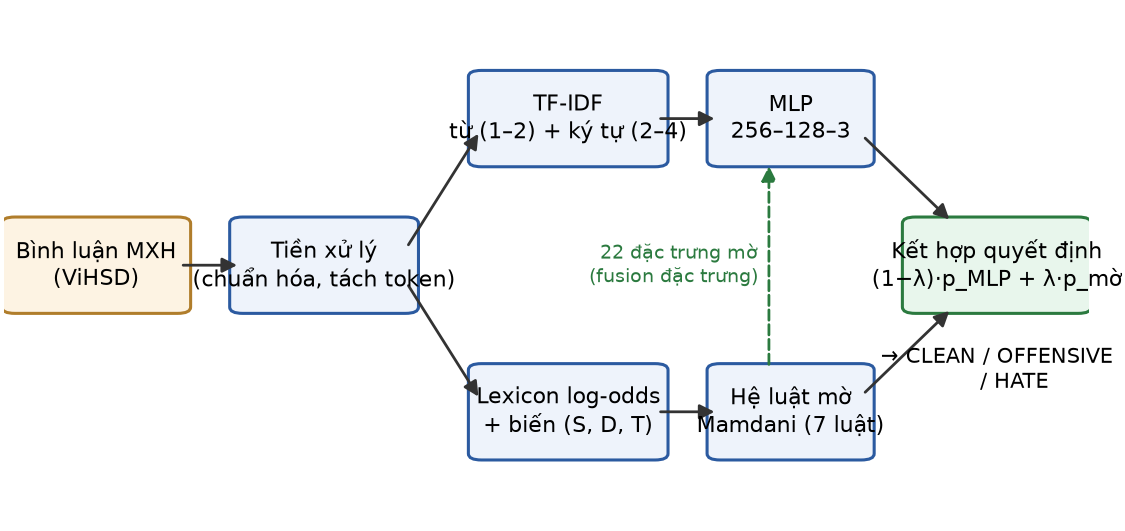
\includegraphics[width=0.98\textwidth]{../outputs/figures/workflow.png}
\figcap{1}{Sơ đồ tổng thể của phương pháp FRF-MLP đề xuất: nhánh trên là kênh thống kê (TF-IDF $\rightarrow$ MLP), nhánh dưới là kênh tri thức (lexicon $\rightarrow$ hệ luật mờ), kết hợp ở mức đặc trưng (mũi tên đứt) và mức quyết định.}
\end{figure}

\subsecvn{3.1. Bước 1: Tiền xử lý và biểu diễn TF-IDF}

\textit{Mục tiêu:} chuyển bình luận thô thành vectơ đặc trưng thống kê. \textit{Đầu vào:} văn bản bình luận. \textit{Đầu ra:} vectơ TF-IDF $\mathbf{x} \in \mathbb{R}^{40022}$ (sau khi nối đặc trưng mờ ở Bước 4).

Văn bản được chuẩn hóa: đưa về chữ thường; thay URL, thẻ người dùng và chữ số bằng token đặc biệt; rút gọn ký tự lặp (ví dụ ``keooooo'' $\rightarrow$ ``keoo''). Chúng tôi \textit{cố ý giữ nguyên} teencode và từ tục viết tắt (``vcl'', ``đm'', ``cc''\ldots) vì chúng là tín hiệu phân loại quan trọng [1]. Văn bản sau đó được biểu diễn bằng hai bộ TF-IDF: mức từ với n-gram (1--2), 20.000 chiều, và mức ký tự trong biên từ với n-gram (2--4), 20.000 chiều. Cách tiếp cận hai mức được chọn vì n-gram ký tự bắt được các biến thể chính tả và teencode mà n-gram từ bỏ sót — đặc điểm cố hữu của văn bản mạng xã hội tiếng Việt.

\subsecvn{3.2. Bước 2: Học từ điển công kích và trích biến ngôn ngữ}

\textit{Mục tiêu:} định lượng mức độ công kích của từng token mà không cần từ điển thủ công. \textit{Đầu vào:} tập huấn luyện đã gán nhãn. \textit{Đầu ra:} điểm $z_w$ cho mỗi token $w$ và ba biến ngôn ngữ $(S, D, T) \in [0,1]^3$ cho mỗi văn bản.

Điểm công kích của token được ước lượng bằng tỷ số log-odds với tiên nghiệm Dirichlet [12], so sánh tần suất của $w$ trong nhóm nhãn $\{$OFFENSIVE, HATE$\}$ (ký hiệu $o$) với nhóm CLEAN (ký hiệu $c$):
\begin{equation}
z_w = \frac{\delta_w}{\sqrt{\dfrac{1}{y_w^{o}+\alpha_w} + \dfrac{1}{y_w^{c}+\alpha_w}}}, \qquad
\delta_w = \log\frac{y_w^{o}+\alpha_w}{n^{o}+\alpha_0-y_w^{o}-\alpha_w} - \log\frac{y_w^{c}+\alpha_w}{n^{c}+\alpha_0-y_w^{c}-\alpha_w}
\end{equation}
trong đó $y_w^{o}, y_w^{c}$ là tần suất của $w$ trong từng nhóm, $n^{o}, n^{c}$ là tổng số token, $\alpha_w$ là tiên nghiệm tỷ lệ với tần suất toàn cục và $\alpha_0 = 1000$. Cách chuẩn hóa phương sai này ổn định hơn PMI với các token hiếm. Các token điểm cao nhất học được gồm ``thằng'', ``ngu'', ``đéo'', ``mày'', ``bọn'' — trùng khớp với trực giác ngôn ngữ, xác nhận chất lượng từ điển.

Từ từ điển, mỗi văn bản được tóm tắt bằng ba biến ngôn ngữ: $S$ — độ công kích cực đại ($\max_w z_w$); $D$ — mật độ từ công kích (tỷ lệ token có $z_w > 2$); $T$ — độ nhắm đích (tỷ lệ đại từ/danh xưng chỉ đối tượng như ``mày'', ``thằng'', ``bọn'', ``lũ''). Biến $T$ được thiết kế riêng để phân biệt HATE (công kích \textit{nhắm đích}) với OFFENSIVE (tục tĩu \textit{không nhắm đích}) theo đúng định nghĩa nhãn của ViHSD [1]. Cả ba được chuẩn hóa về $[0,1]$ theo phân vị 5--95 của tập huấn luyện.

\subsecvn{3.3. Bước 3: Suy diễn mờ Mamdani}

\textit{Mục tiêu:} chuyển $(S,D,T)$ thành độ kích hoạt luật và phân phối lớp mờ có thể diễn giải. \textit{Đầu vào:} $(S,D,T)$. \textit{Đầu ra:} vectơ đặc trưng mờ $\mathbf{f} \in \mathbb{R}^{22}$ và phân phối $\mathbf{p}^{\mathrm{fuzzy}} \in \Delta^2$.

Mỗi biến được mờ hóa bằng ba hàm thành viên hình thang LOW/MED/HIGH (Hình 2):
\begin{equation}
\mu_{[a,b,c,d]}(v) = \max\!\Big(0,\ \min\!\Big(\frac{v-a}{b-a},\ 1,\ \frac{d-v}{d-c}\Big)\Big)
\end{equation}
Bảy luật Mamdani (Bảng 1) được suy diễn bằng t-norm min; ví dụ luật R5: \textit{NẾU $S$ là HIGH VÀ $T$ là MED hoặc HIGH THÌ lớp là HATE}. Độ kích hoạt của luật $k$ với hệ số tin cậy $w_k$ là:
\begin{equation}
r_k = w_k \cdot \min_{j \in A_k} \mu_j(\mathbf{v}), \qquad
p^{\mathrm{fuzzy}}_c = \frac{\sum_{k:\, \mathrm{cons}(k)=c} r_k + b_c}{\sum_{c'}\big(\sum_{k:\, \mathrm{cons}(k)=c'} r_k + b_{c'}\big)}
\end{equation}
trong đó $A_k$ là tập mệnh đề điều kiện của luật $k$ và $b_c$ là thiên lệch nhỏ về CLEAN khi không luật nào kích hoạt. Vectơ đặc trưng mờ đầy đủ $\mathbf{f} = [S,D,T \,\|\, \boldsymbol{\mu} \,\|\, \mathbf{r} \,\|\, \mathbf{p}^{\mathrm{fuzzy}}] \in \mathbb{R}^{22}$ gồm 3 biến gốc, 9 độ thuộc, 7 độ kích hoạt luật và 3 xác suất mờ.

\begin{table}[!htb]
\tabcap{1}{Hệ bảy luật mờ Mamdani của FRF-MLP (t-norm min; $w_k$ là hệ số tin cậy).}
\centering
{\fontsize{10}{12}\selectfont
\begin{tabular}{@{}llll@{}}
\toprule
Luật & Điều kiện & Kết luận & $w_k$\\
\midrule
R1 & $S$ LOW $\wedge$ $D$ LOW & CLEAN & 1,0\\
R2 & $S$ MED $\wedge$ $T$ LOW & OFFENSIVE & 1,0\\
R3 & $S$ HIGH $\wedge$ $T$ LOW & OFFENSIVE & 1,0\\
R4 & $S$ MED $\wedge$ $T$ HIGH & HATE & 0,9\\
R5 & $S$ HIGH $\wedge$ ($T$ MED $\vee$ $T$ HIGH) & HATE & 1,0\\
R6 & $D$ HIGH $\wedge$ $T$ HIGH & HATE & 0,8\\
R7 & $D$ MED $\wedge$ $T$ LOW & OFFENSIVE & 0,7\\
\bottomrule
\end{tabular}}
\end{table}

\begin{figure}[!htb]
\centering
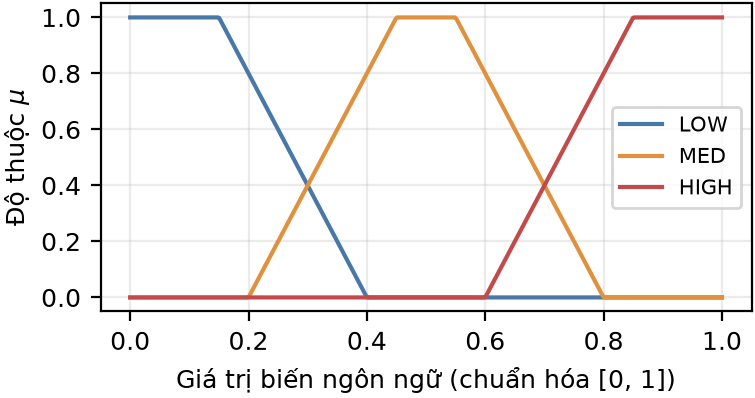
\includegraphics[width=0.62\textwidth]{../outputs/figures/memberships.png}
\figcap{2}{Ba hàm thành viên hình thang LOW/MED/HIGH dùng chung cho ba biến ngôn ngữ $S$, $D$, $T$ sau chuẩn hóa.}
\end{figure}

\subsecvn{3.4. Bước 4: MLP và kết hợp hai mức}

\textit{Mục tiêu:} hợp nhất kênh thống kê và kênh tri thức. \textit{Đầu vào:} $\mathbf{x}$ (TF-IDF), $\mathbf{f}$, $\mathbf{p}^{\mathrm{fuzzy}}$. \textit{Đầu ra:} phân phối lớp cuối cùng $\mathbf{p}$.

\textit{Kết hợp mức đặc trưng:} đầu vào MLP là $[\mathbf{x} \,\|\, \mathbf{f}] \in \mathbb{R}^{40022}$. MLP có hai lớp ẩn 256--128 với ReLU và dropout:
\begin{equation}
\mathbf{h}_1 = \mathrm{ReLU}(\mathbf{W}_1 [\mathbf{x} \| \mathbf{f}] + \mathbf{b}_1), \quad
\mathbf{h}_2 = \mathrm{ReLU}(\mathbf{W}_2 \mathbf{h}_1 + \mathbf{b}_2), \quad
\mathbf{p}^{\mathrm{MLP}} = \mathrm{softmax}(\mathbf{W}_3 \mathbf{h}_2 + \mathbf{b}_3)
\end{equation}
Mạng được huấn luyện bằng lan truyền ngược [4] với hàm mất mát entropy chéo có trọng số lớp $n/(3 n_c)$ để xử lý mất cân bằng nhãn.

\textit{Kết hợp mức quyết định:} phân phối cuối cùng là tổ hợp lồi
\begin{equation}
\mathbf{p} = (1-\lambda)\, \mathbf{p}^{\mathrm{MLP}} + \lambda\, \mathbf{p}^{\mathrm{fuzzy}}, \qquad \lambda \in [0,1]
\end{equation}
với $\lambda$ được quét trên lưới $\{0; 0{,}05; \ldots; 1\}$ và chọn theo macro-F1 trên tập phát triển. Cơ chế hai mức là cần thiết vì chúng bổ trợ: mức đặc trưng cho phép MLP \textit{học} tương tác phi tuyến giữa tín hiệu mờ và TF-IDF, còn mức quyết định giữ lại ảnh hưởng \textit{tường minh} của hệ luật ngay cả khi MLP quá khớp. Thuật toán 1 tóm tắt toàn bộ quy trình, thể hiện liên kết đầu vào--đầu ra giữa bốn bước.

\begin{table}[!htb]
\centering
{\fontsize{10}{12}\selectfont
\begin{tabular}{@{}p{15.2cm}@{}}
\toprule
\textbf{Thuật toán 1.} FRF-MLP: huấn luyện và suy diễn\\
\midrule
\textbf{Đầu vào:} tập huấn luyện $\mathcal{D}_{tr}=\{(t_i,y_i)\}$, tập phát triển $\mathcal{D}_{dev}$, văn bản kiểm tra $t$\\
\textbf{Đầu ra:} nhãn dự đoán $\hat{y}(t) \in \{$CLEAN, OFFENSIVE, HATE$\}$\\[2pt]
1: \textbf{(B1)} Chuẩn hóa mọi văn bản; khớp hai bộ TF-IDF trên $\mathcal{D}_{tr}$ $\Rightarrow$ ánh xạ $t \mapsto \mathbf{x}(t)$\\
2: \textbf{(B2)} Tính $z_w$ theo (1) trên $\mathcal{D}_{tr}$; khớp phân vị 5--95 $\Rightarrow$ ánh xạ $t \mapsto (S,D,T)(t)$\\
3: \textbf{(B3)} Với mỗi $t$: tính $\boldsymbol{\mu}$ theo (2), $\mathbf{r}, \mathbf{p}^{\mathrm{fuzzy}}$ theo (3) $\Rightarrow$ $\mathbf{f}(t) \in \mathbb{R}^{22}$\\
4: \textbf{(B4a)} Huấn luyện MLP (4) trên $\{([\mathbf{x}\|\mathbf{f}](t_i), y_i)\}$, dừng sớm theo macro-F1 trên $\mathcal{D}_{dev}$\\
5: \textbf{(B4b)} $\lambda^{*} \leftarrow \arg\max_{\lambda} \mathrm{macroF1}\big(\mathcal{D}_{dev};\ (1-\lambda)\mathbf{p}^{\mathrm{MLP}} + \lambda \mathbf{p}^{\mathrm{fuzzy}}\big)$\\
6: \textbf{Suy diễn:} $\hat{y}(t) = \arg\max_c \big[(1-\lambda^{*})\, p^{\mathrm{MLP}}_c(t) + \lambda^{*} p^{\mathrm{fuzzy}}_c(t)\big]$ theo (5)\\
\bottomrule
\end{tabular}}
\vspace{2pt}
\end{table}

% ============================ 4. THUC NGHIEM ============================
\secvn{4. Kết quả thực nghiệm}

\subsecvn{4.1. Chuẩn bị tập dữ liệu}

Chúng tôi dùng ViHSD [1] — bộ dữ liệu chuẩn lớn nhất cho bài toán này — gồm 33.398 bình luận Facebook/YouTube có nhãn, chia sẵn train/dev/test theo tỷ lệ 7--1--2: 24.046 mẫu huấn luyện, 2.672 mẫu phát triển và 6.680 mẫu kiểm tra. Việc giữ nguyên phép chia gốc của tác giả bộ dữ liệu bảo đảm kết quả so sánh được trực tiếp với các nghiên cứu đã công bố. Phân bố nhãn (Hình 3) mất cân bằng nặng: CLEAN chiếm 82,7\%, OFFENSIVE 6,7\%, HATE 10,6\% — lý do macro-F1 được chọn làm thước đo chính thay vì accuracy. Về EDA và chuẩn hóa: chúng tôi khảo sát độ dài, tỷ lệ teencode và phân bố nhãn theo split; chuẩn hóa nhẹ như mô tả ở Mục 3.1 (không xóa từ dừng, không tách từ ghép) vì các thao tác nặng tay làm mất tín hiệu công kích.

\begin{figure}[!htb]
\centering
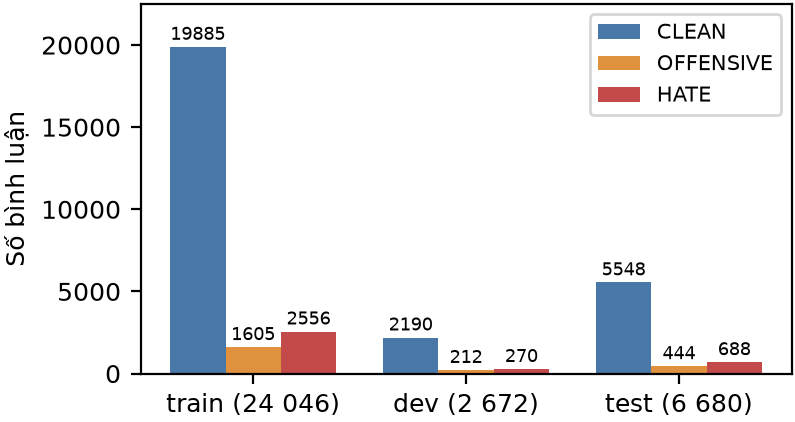
\includegraphics[width=0.6\textwidth]{../outputs/figures/label_dist.png}
\figcap{3}{Phân bố ba nhãn trên các tập train, dev, test của ViHSD.}
\end{figure}

\subsecvn{4.2. Thiết lập thực nghiệm}

Bảng 2 liệt kê toàn bộ siêu tham số. Các giá trị TF-IDF và kiến trúc MLP theo thông lệ; $\alpha_0$, ngưỡng $z$, và biên hàm thành viên chọn theo khảo sát sơ bộ trên tập phát triển; $\lambda$ quét lưới trên tập phát triển. Mọi thực nghiệm dùng seed 42, chạy trên CPU AMD Ryzen 9 9950X3D (PyTorch 2.13, scikit-learn 1.9); mỗi mô hình MLP huấn luyện dưới hai phút.

Các phương pháp so sánh gồm: (i) baseline nội bộ — hệ mờ thuần (chỉ $\mathbf{p}^{\mathrm{fuzzy}}$), hồi quy softmax (mô hình tuyến tính có trọng số lớp, $C$ chọn trên tập phát triển trong $\{0{,}25; 0{,}5; 1; 2; 4; 8\}$), MLP thuần; (ii) kết quả đã công bố trên cùng phép chia ViHSD [1] — Text-CNN, GRU (embedding fastText), m-BERT, XLM-R, DistilBERT. Các phương pháp ablation gồm: MLP + kết hợp quyết định (bỏ mức đặc trưng) và MLP + đặc trưng mờ (bỏ mức quyết định).

\begin{table}[!htb]
\tabcap{2}{Thiết lập siêu tham số của các thực nghiệm.}
\centering
{\fontsize{10}{12}\selectfont
\begin{tabular}{@{}llll@{}}
\toprule
Thành phần & Tham số & Thành phần & Tham số\\
\midrule
TF-IDF từ & n-gram (1--2), 20.000 chiều, min\_df 2 & MLP & 2 lớp ẩn 256--128, ReLU, dropout 0,3\\
TF-IDF ký tự & char\_wb (2--4), 20.000 chiều & Tối ưu & AdamW, lr $10^{-3}$, weight decay $10^{-4}$\\
Lexicon & $\alpha_0=1000$, tần suất tối thiểu 3 & Batch/epoch & 256 / tối đa 40, dừng sớm patience 5\\
Biến mờ & ngưỡng $z>2$; phân vị 5--95 & Trọng số lớp & $n/(3n_c)$\\
Hàm thành viên & hình thang, biên như Hình 2 & $\lambda$ & lưới $\{0; 0{,}05; \ldots; 1\}$ theo dev\\
\bottomrule
\end{tabular}}
\end{table}

\subsecvn{4.3. Đánh giá kết quả đạt được}

\subsubsecvn{4.3.1. Kết quả của phương pháp đề xuất}

FRF-MLP đạt 84,46\% accuracy, 62,95\% macro-F1 và 84,81\% F1 có trọng số trên tập kiểm tra, với $\lambda^{*} = 0{,}25$. Bảng 3 nêu chi tiết theo lớp: mô hình giữ độ chính xác cao ở CLEAN (F1 91,9\%) đồng thời đạt recall 45,0\% cho OFFENSIVE và 56,4\% cho HATE — hai lớp thiểu số vốn khó nhất. Hình 4a cho thấy đặc trưng mờ giúp mô hình khởi động tốt hơn hẳn (macro-F1 dev 60,1\% ngay epoch đầu so với 57,2\% của MLP thuần); Hình 4b cho thấy macro-F1 dev đạt đỉnh quanh $\lambda \in [0{,}15; 0{,}30]$ rồi giảm mạnh khi hệ mờ lấn át — đúng kỳ vọng: hệ luật chỉ nên đóng vai trò \textit{hiệu chỉnh} quyết định của MLP.

\begin{table}[!htb]
\tabcap{3}{Kết quả chi tiết theo lớp của FRF-MLP trên tập kiểm tra ViHSD (\%).}
\centering
{\fontsize{10}{12}\selectfont
\begin{tabular}{@{}lcccc@{}}
\toprule
Lớp & Precision & Recall & F1 & Số mẫu\\
\midrule
CLEAN & 92,8 & 91,1 & 91,9 & 5.548\\
OFFENSIVE & 38,8 & 45,0 & 41,7 & 444\\
HATE & 54,2 & 56,4 & 55,3 & 688\\
\midrule
Accuracy / Macro-F1 / Weighted-F1 & \multicolumn{4}{c}{84,46 / 62,95 / 84,81}\\
\bottomrule
\end{tabular}}
\end{table}

\begin{figure}[!htb]
\centering

\includegraphics[width=0.98\textwidth]{../outputs/figures/training.png}
\figcap{4}{(a) Macro-F1 trên tập dev theo epoch của MLP thuần và MLP + đặc trưng mờ; (b) macro-F1 trên tập dev khi quét trọng số kết hợp $\lambda$.}
\end{figure}

\subsubsecvn{4.3.2. So sánh với các phương pháp khác}

Bảng 4 so sánh với các kết quả đã công bố trên cùng phép chia ViHSD (thừa nhận lại số liệu từ [1]) và các baseline nội bộ; Hình 5 trực quan hóa nhóm nội bộ. Về macro-F1 — thước đo phù hợp với dữ liệu mất cân bằng — FRF-MLP (62,95\%) vượt mọi mô hình đã công bố, kể cả m-BERT cased (62,69\%), trong khi chỉ dùng ${\sim}10{,}3$ triệu tham số huấn luyện từ đầu trên CPU, so với ${\sim}178$ triệu tham số tiền huấn luyện đa ngữ của m-BERT. Accuracy của FRF-MLP thấp hơn nhóm Transformer (84,46\% so với 86,88\%): đây là đánh đổi có chủ đích của trọng số lớp — chấp nhận giảm nhẹ độ chính xác trên lớp đa số CLEAN để tăng recall các lớp thiểu số, mục tiêu thực tế của hệ kiểm duyệt.

Đáng chú ý, hồi quy softmax có trọng số lớp là baseline rất mạnh về macro-F1 (64,50\%) — vượt cả các mô hình sâu, một hiện tượng đã biết trên không gian TF-IDF thưa chiều cao, nơi mô hình tuyến tính lồi hội tụ toàn cục còn MLP dễ quá khớp. Điều này không phủ nhận đóng góp của nghiên cứu: câu hỏi nghiên cứu đặt ra là \textit{tri thức mờ có cải thiện MLP hay không}, và kết quả ablation (Mục 4.3.3) trả lời khẳng định với mức cải thiện nhất quán; việc áp cùng cơ chế kết hợp mờ lên các bộ phân loại khác là hướng mở tự nhiên.

\begin{table}[!htb]
\tabcap{4}{So sánh trên tập kiểm tra ViHSD. Nhóm trên: kết quả đã công bố [1]; nhóm dưới: thực nghiệm của nghiên cứu này (cùng phép chia dữ liệu).}
\centering
{\fontsize{10}{12}\selectfont
\begin{tabular}{@{}llcc@{}}
\toprule
Mô hình & Nguồn & Accuracy (\%) & Macro-F1 (\%)\\
\midrule
Text-CNN (fastText) & [1] & 86,69 & 61,11\\
GRU (fastText) & [1] & 85,41 & 60,47\\
m-BERT uncased & [1] & 86,60 & 62,38\\
m-BERT cased & [1] & \textbf{86,88} & 62,69\\
XLM-R base & [1] & 86,12 & 61,28\\
DistilBERT đa ngữ & [1] & 86,22 & 62,42\\
\midrule
Hệ mờ thuần & nghiên cứu này & 53,28 & 41,56\\
Hồi quy softmax (trọng số lớp) & nghiên cứu này & 84,79 & \textbf{64,50}\\
MLP thuần & nghiên cứu này & 83,80 & 61,03\\
FRF-MLP (đề xuất) & nghiên cứu này & 84,46 & 62,95\\
\bottomrule
\end{tabular}}
\end{table}

\begin{figure}[!htb]
\centering
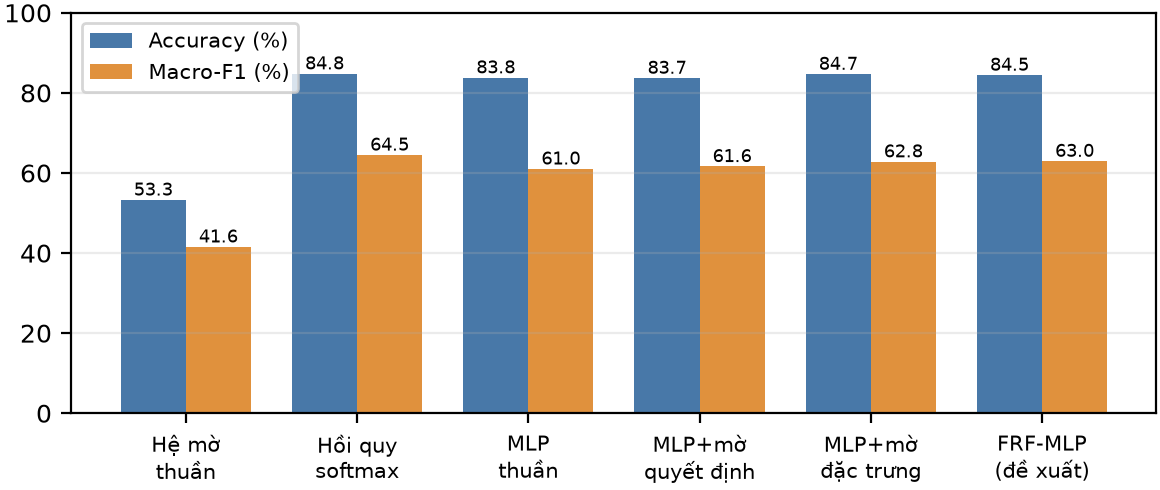
\includegraphics[width=0.95\textwidth]{../outputs/figures/comparison.png}
\figcap{5}{Accuracy và macro-F1 trên tập kiểm tra của các mô hình thực nghiệm trong nghiên cứu này.}
\end{figure}

\subsubsecvn{4.3.3. Kết quả các phương pháp ablation}

Bảng 5 tách đóng góp của từng mức kết hợp. Riêng mức quyết định (+0,61 macro-F1) hay riêng mức đặc trưng (+1,79) đều cải thiện MLP thuần; kết hợp cả hai đạt +1,92. Hệ mờ thuần chỉ đạt 41,56\% macro-F1 — quá yếu để đứng một mình nhưng \textit{bổ sung} hiệu quả: ma trận nhầm lẫn (Hình 6) cho thấy FRF-MLP tăng recall OFFENSIVE từ 40,5\% lên 45,0\% và HATE từ 54,7\% lên 56,4\% so với MLP thuần, đồng thời giảm 36 trường hợp OFFENSIVE bị nhầm sang HATE (101 $\rightarrow$ 75) — đúng vùng mà biến nhắm đích $T$ được thiết kế để phân giải. Điều này khẳng định giả thuyết trung tâm: tri thức ngôn ngữ mờ và thống kê TF-IDF mang thông tin bổ trợ, không trùng lặp.

\begin{table}[!htb]
\tabcap{5}{Kết quả ablation trên tập kiểm tra ViHSD (\%). $\Delta$ tính theo macro-F1 so với MLP thuần.}
\centering
{\fontsize{10}{12}\selectfont
\begin{tabular}{@{}lccc@{}}
\toprule
Cấu hình & Accuracy & Macro-F1 & $\Delta$\\
\midrule
MLP thuần (gốc ablation) & 83,80 & 61,03 & ---\\
MLP + kết hợp quyết định ($\lambda^{*}=0{,}20$) & 83,70 & 61,64 & +0,61\\
MLP + đặc trưng mờ & 84,69 & 62,82 & +1,79\\
FRF-MLP đầy đủ ($\lambda^{*}=0{,}25$) & 84,46 & 62,95 & +1,92\\
\bottomrule
\end{tabular}}
\end{table}

\begin{figure}[!htb]
\centering

\includegraphics[width=0.9\textwidth]{../outputs/figures/confusion.png}
\figcap{6}{Ma trận nhầm lẫn trên tập kiểm tra: (a) MLP thuần; (b) FRF-MLP đề xuất. Giá trị trong ngoặc là tỷ lệ theo hàng.}
\end{figure}

% ============================ 5. KET LUAN ============================
\secvn{5. Kết luận}

Nghiên cứu đã đề xuất FRF-MLP — mô hình kết hợp MLP với hệ luật mờ Mamdani ở hai mức đặc trưng và quyết định — cho bài toán phát hiện ngôn từ công kích trên văn bản mạng xã hội tiếng Việt. Toàn bộ thành phần mờ (từ điển log-odds, biến ngôn ngữ, luật) được xây dựng tự động từ dữ liệu huấn luyện, không cần từ điển thủ công. Trên ViHSD, phương pháp đạt 84,46\% accuracy và 62,95\% macro-F1, cải thiện +1,92 điểm macro-F1 so với MLP thuần và vượt các baseline đã công bố (Text-CNN, GRU, họ BERT đa ngữ) về macro-F1 với chi phí huấn luyện chỉ vài phút CPU.

Ưu điểm của phương pháp là nhẹ, diễn giải được ở mức luật, và cải thiện nhất quán các lớp thiểu số. Hạn chế: hệ mờ đứng một mình còn yếu; hồi quy softmax có trọng số lớp vẫn nhỉnh hơn về macro-F1, cho thấy kiến trúc MLP trên TF-IDF thưa chưa phải bộ học tối ưu; biên hàm thành viên đang cố định thủ công. Hướng phát triển: (i) học biên hàm thành viên và trọng số luật đầu-cuối theo tinh thần ANFIS [9]; (ii) thay TF-IDF bằng embedding PhoBERT [6] làm đầu vào cho FRF-MLP; (iii) áp cơ chế kết hợp mờ hai mức lên các bộ phân loại khác và các bộ dữ liệu tiếng Việt khác như VLSP-HSD [3].

\secvn{Xung đột lợi ích}

\noindent Các tác giả tuyên bố không có xung đột lợi ích trong bài báo này.

\secvn{Tuyên bố dữ liệu sẵn có}

\noindent Bộ dữ liệu ViHSD được công bố công khai bởi nhóm tác giả [1]. Mã nguồn thực nghiệm của nghiên cứu này được cung cấp khi độc giả yêu cầu một cách hợp lý.

% ============================ TAI LIEU THAM KHAO ============================
\secvn{TÀI LIỆU THAM KHẢO}

{\fontsize{8}{10}\selectfont
\setlength{\parindent}{0cm}
\newenvironment{refitem}{\par\hangindent=0.75cm\hangafter=1\noindent}{}

\begin{refitem}[1] S. T. Luu, K. V. Nguyen, and N. L.-T. Nguyen, ``A large-scale dataset for hate speech detection on Vietnamese social media texts,'' in \textit{Proc. 34th Int. Conf. Industrial, Engineering and Other Applications of Applied Intelligent Systems (IEA/AIE)}, Kuala Lumpur, Malaysia, 2021, pp. 415--426, doi: 10.1007/978-3-030-79457-6\_35.\end{refitem}
\begin{refitem}[2] T. Davidson, D. Warmsley, M. Macy, and I. Weber, ``Automated hate speech detection and the problem of offensive language,'' in \textit{Proc. 11th Int. AAAI Conf. Web and Social Media (ICWSM)}, Montreal, Canada, 2017, pp. 512--515.\end{refitem}
\begin{refitem}[3] X.-S. Vu, T. Vu, M.-V. Tran, T. Le-Cong, and H. T. M. Nguyen, ``HSD shared task in VLSP campaign 2019: Hate speech detection for social good,'' arXiv preprint arXiv:2007.06493, 2020.\end{refitem}
\begin{refitem}[4] D. E. Rumelhart, G. E. Hinton, and R. J. Williams, ``Learning representations by back-propagating errors,'' \textit{Nature}, vol. 323, no. 6088, pp. 533--536, Oct. 1986, doi: 10.1038/323533a0.\end{refitem}
\begin{refitem}[5] J. Devlin, M.-W. Chang, K. Lee, and K. Toutanova, ``BERT: Pre-training of deep bidirectional transformers for language understanding,'' in \textit{Proc. NAACL-HLT}, Minneapolis, MN, USA, 2019, pp. 4171--4186, doi: 10.18653/v1/N19-1423.\end{refitem}
\begin{refitem}[6] D. Q. Nguyen and A. T. Nguyen, ``PhoBERT: Pre-trained language models for Vietnamese,'' in \textit{Findings of the Association for Computational Linguistics: EMNLP 2020}, 2020, pp. 1037--1042, doi: 10.18653/v1/2020.findings-emnlp.92.\end{refitem}
\begin{refitem}[7] L. A. Zadeh, ``Fuzzy sets,'' \textit{Information and Control}, vol. 8, no. 3, pp. 338--353, Jun. 1965, doi: 10.1016/S0019-9958(65)90241-X.\end{refitem}
\begin{refitem}[8] L.-X. Wang and J. M. Mendel, ``Generating fuzzy rules by learning from examples,'' \textit{IEEE Trans. Syst., Man, Cybern.}, vol. 22, no. 6, pp. 1414--1427, Nov./Dec. 1992, doi: 10.1109/21.199466.\end{refitem}
\begin{refitem}[9] J.-S. R. Jang, ``ANFIS: Adaptive-network-based fuzzy inference system,'' \textit{IEEE Trans. Syst., Man, Cybern.}, vol. 23, no. 3, pp. 665--685, May/Jun. 1993, doi: 10.1109/21.256541.\end{refitem}
\begin{refitem}[10] Y. Deng, Z. Ren, Y. Kong, F. Bao, and Q. Dai, ``A hierarchical fused fuzzy deep neural network for data classification,'' \textit{IEEE Trans. Fuzzy Syst.}, vol. 25, no. 4, pp. 1006--1012, Aug. 2017, doi: 10.1109/TFUZZ.2016.2574915.\end{refitem}
\begin{refitem}[11] S. Vashishtha and S. Susan, ``Fuzzy rule based unsupervised sentiment analysis from social media posts,'' \textit{Expert Syst. Appl.}, vol. 138, Dec. 2019, Art. no. 112834, doi: 10.1016/j.eswa.2019.112834.\end{refitem}
\begin{refitem}[12] B. L. Monroe, M. P. Colaresi, and K. M. Quinn, ``Fightin' words: Lexical feature selection and evaluation for identifying the content of political conflict,'' \textit{Political Analysis}, vol. 16, no. 4, pp. 372--403, 2008, doi: 10.1093/pan/mpn018.\end{refitem}
}

% ============================ TIEU SU ============================
\vspace{10pt}
\secvn{TÓM TẮT TIỂU SỬ TÁC GIẢ}

\noindent
\begin{tabular}{@{}p{15.9cm}@{}}
\textbf{Anh Tu Phuong Nguyen} (family name: Nguyen) received the B.Eng. degree in Information Technology from Ho Chi Minh City University of Technology and Education (HCMUTE), Ho Chi Minh City, Vietnam. He is currently a Master's student in Computer Science at HCMUTE (student ID 2611328).\\[3pt]
He has industry experience as a software and AI engineer, working on production web systems and applied machine learning products in Ho Chi Minh City, Vietnam.\\[3pt]
His research interests include machine learning, natural language processing, neuro-fuzzy systems, hate speech detection, and Vietnamese text classification.\\[3pt]
Email: 2611328@student.hcmute.edu.vn. ORCID: https://orcid.org/0000-000X-XXXX-XXXX.\\
\end{tabular}

\end{document}
